\begin{name}
	{\tenchude}{ĐỀ ÔN TẬP SỐ 8}{LỚP TOÁN THẦY PHÁT}{\thoigian}
\end{name}
\setcounter{ex}{0}
\setcounter{bt}{0}
\Opensolutionfile{ans}[ans/ans-Vted-18-2023]
%%==========Câu 1
\begin{ex}%[2D4B1-2]%[Nguyen Huynh]%[Đề thi thử Vted Năm 2023]
	\immini{
		Trong mặt phẳng tọa độ $Oxy$, cho các điểm $M, N, P, Q$ như bên cạnh, số phức $z=1-4i$ được biểu diễn bởi điểm
		\choice
		{$N$}
		{$P$}
		{$Q$}
		{\True $M$}}{
		\begin{tikzpicture}[thick,>=stealth,scale=0.65]
			\draw[->] (-5,0) -- (5,0) node[above] {\small $x$};
			\draw[->] (0,-5) -- (0,4.5) node[right] {\small $y$};
			\draw[dashed] (1,0)--(1,-4)--(0,-4)--(0,4)--(-1,4)--(-1,0);
			\draw[dashed]
			(-4,0)--(-4,1)--(4,1)--(4,0);
			\draw[fill=black] (1,-4) node [above right]{\footnotesize $M$} circle (0.05);
			\draw[fill=black] (4,1) node [above left]{\footnotesize $N$} circle (0.05);
			\draw[fill=black] (-4,1) node [above right]{\footnotesize $Q$} circle (0.05);
			\draw[fill=black] (-1,4) node [below left]{\footnotesize $P$} circle (0.05);
			\draw[fill=black] (4,0) node [below left]{\footnotesize $4$} circle (0.001);
			\draw[fill=black] (-4,0) node [below left]{\footnotesize $-4$} circle (0.001);
			\draw[fill=black] (1,0) node [below left]{\footnotesize $1$} circle (0.005);
			\draw[fill=black] (-1,0) node [below left]{\footnotesize $-1$} circle (0.005);
			\draw[fill=black] (0,1) node [above left]{\footnotesize $1$} circle (0.005);
			\draw[fill=black] (0,4) node [below right]{\footnotesize $4$} circle (0.005);
			\draw[fill=black] (0,-4) node [above left]{\footnotesize $-4$} circle (0.005);
	\end{tikzpicture}}
	
	\loigiai{Theo hình vẽ, ta có điểm biểu diễn số phức $z=1-4i$ là điểm $M(1;-4)$.
		
	}
\end{ex}

%%==========Câu 2
\begin{ex}%[2D1Y2-2]%[Nguyen Huynh]%[Đề thi thử Vted Năm 2023]
	Cho hàm số $y=f(x)$ có bảng xét dấu của đạo hàm như sau
	\begin{center}
		
\begin{tikzpicture}
			\tkzTabInit[espcl=2.5,lgt=1]
			{$x$/0.7,$f'(x)$/0.7}
			{$-\infty$,$-2$,$0$,$1$,$4$,$+\infty$}
			\tkzTabLine{,+,z,-,z,+,z,-,z,+,}
		\end{tikzpicture}
	\end{center}
	Số điểm cực trị của hàm số đã cho là
	\choice
	{$3$}
	{$2$}
	{\True $4$}
	{$5$}
	\loigiai{
		Ta có $f'(x)$ đổi dấu $4$ lần nên có $4$ điểm cực trị.
	}
\end{ex}

%%==========Câu 3
\begin{ex}%[2H2Y2-1]%[Nguyen Huynh]%[Đề thi thử Vted Năm 2023]
	Thể tích của khối cầu có bán kính $r=3$ bằng
	\choice
	{$9\pi$}
	{$4\pi^3$}
	{$108\pi$}
	{\True $36\pi$}
	\loigiai{
		Ta có $V=\dfrac{4}{3}\pi R^3=\dfrac{4\pi}{3}\cdot 27 = 36\pi$.
	}
\end{ex}

%%==========Câu 4
\begin{ex}%[2D3Y1-1]%[Nguyen Huynh]%[Đề thi thử Vted Năm 2023]
	Số phức liên hợp của số phức $z=5-2i$ là
	\choice
	{\True $\overline{z}=5+2i$}
	{$\overline{z}=2+5i$}
	{$\overline{z}=-5-2i$}
	{$\overline{z}=-2-5i$}
	\loigiai{Số phức liên hợp của số phức $z=5-2i$ là $\overline{z}=5+2i$.
	}
\end{ex}

%%==========Câu 5
\begin{ex}%[2H3Y1-3]%[Nguyen Huynh]%[Đề thi thử Vted Năm 2023]
	Trong KG $Oxyz$, cho mặt cầu $(S)$ có tâm $I(1;0;2)$ và bán kính $R=3$. Phương trình của mặt cầu $(S)$ là 
	\choice
	{$(x+1)^2+y^2+(z+2)^2=3$}
	{$(x-1)^2+y^2+(z-2)^2=3$}
	{$(x+1)^2+y^2+(z-2)^2=9$}
	{\True $(x-1)^2+y^2+(z-2)^2=9$}
	\loigiai{Mặt cầu $(S)$ có tâm $I(1;0;2)$ và bán kính $R=3$ nên có phương trình là $(S)\colon (x-1)^2+y^2+(z-2)^2=9$.
	}
\end{ex}

%%==========Câu 6
\begin{ex}%[2D1Y5-7]%[Nguyen Huynh]%[Đề thi thử Vted Năm 2023]
	Đồ thị của hàm số $y=\dfrac{x+1}{x-1}$ cắt trục $Ox$ tại điểm nào dưới đây?
	\choice
	{$M(0;-1)$}
	{\True $N(-1;0)$}
	{$P(0;1)$}
	{$Q(1;0)$}
	\loigiai{
		Ta có $\dfrac{x+1}{x-1}=0 \Leftrightarrow x=-1$.\\ Do đó  hàm số đã cho cắt trục $Ox$ tại $N(-1;0)$.}
\end{ex}
%%==========Câu 7
\begin{ex} %[2D1Y1-2]%[Nguyen Huynh]%[Đề thi thử Vted Năm 2023]
	Cho hàm số $y=f(x)$ có bảng biến thiên như sau
	\begin{center}
		
\begin{tikzpicture}[font=\footnotesize,line join= round,line cap=round,>=stealth,scale=.8]
			\tkzTabInit[nocadre=false,lgt=0.7,espcl=2.5,deltacl=0.6pt]
			{$x$ /.6,$y'$ /.6,$y$ /2}
			{$-\infty$,$1$,$3$,$+\infty$}
			\tkzTabLine{,+,$0$,-,$0$,+,}
			\tkzTabVar{-/ $-\infty$,+/$2$,-/$-2$,+/$+\infty$}
		\end{tikzpicture}
	\end{center}
	Hàm số đã cho đồng biến trên khoảng nào dưới đây?
	\choice
	{$(-\infty;2)$}
	{\True $(-\infty;1)$}
	{$(1;+\infty)$}
	{ $(1;3)$}
	
	\loigiai{
		Hàm số đã cho đồng biến trên $(-\infty;1)$.
	}
\end{ex}
%%==========Câu 8
\begin{ex}%[2D4Y1-1]%[Nguyen Huynh]%[Đề thi thử Vted Năm 2023]
	Phần ảo của số phức $z=5-2i$ là
	\choice
	{$2i$}
	{$-2i$}
	{\True$-2$}
	{$2$}
	\loigiai{Phần ảo của số phức $z=5-2i$ là $-2$.}
\end{ex}
%%==========Câu 9
\begin{ex}%[2D2Y6-1]%[Nguyen Huynh]%[Đề thi thử Vted Năm 2023]
	Tập nghiệm của bất phương trình $\log_2(x - 2) > 2$ là 
	\choice
	{$\left(4;+\infty\right)$}
	{$\left(2;+\infty\right)$}
	{\True $\left(6;+\infty\right)$}
	{$\left(2;6\right)$}
	\loigiai{
		Ta có $\log_2(x - 2) > 2\Leftrightarrow x - 2 > 2^2\Leftrightarrow x > 6$. 
	}
\end{ex}

%%==========Câu 10
\begin{ex}%[2D2Y5-1]%[Nguyen Huynh]%[Đề thi thử Vted Năm 2023]
	Nghiệm của phương trình $2^{2x} = 8$ là
	\choice
	{\True $x=\dfrac{3}{2}$}
	{$x=\dfrac{2}{3}$}
	{$x=2$}
	{$x=3$}
	\loigiai{
		Ta có $2^{2x}=8\Leftrightarrow 2x=\log_2 8=3 \Leftrightarrow x=\dfrac{3}{2}$. 
	}
\end{ex}
%%==========Câu 11
\begin{ex}%[Đề thi thử Vted 18 Năm 2023-Nguyễn Thắng]%[2H1Y3-2]
	Thể tích của khối hộp có chiều cao $h=5$, diện tích đáy $B=3$ bằng
	\choice
	{\True $15$}
	{$5$}
	{$5\pi$}
	{$\dfrac{15}{2}$}
	\loigiai{
		Thể tích của khối hộp có chiều cao $h=5$, diện tích đáy $B=3$ là $V=Bh=15$.
	}
\end{ex}

%%==========Câu 12
\begin{ex}%[Đề thi thử Vted 18 Năm 2023-Nguyễn Thắng]%[2D3Y2-1]
	Cho $f(2)=4$, $f(0)=1$, khi đó $\displaystyle\int\limits_0^2f'(x)\mathrm{d}x$ bằng
	\choice
	{$4$}
	{$2$}
	{$5$}
	{\True $3$}
	\loigiai{
		Ta có $\displaystyle\int\limits_0^2f'(x)\mathrm{d}x=f(x)\bigg|_0^2=f(2)-f(0)=4-1=3$.
	}
\end{ex}

%%==========Câu 13
\begin{ex}%[Đề thi thử Vted 18 Năm 2023-Nguyễn Thắng]%[2D1Y5-1]
	Đồ thị của hàm số nào dưới đây có dạng như đường cong trong hình bên?
	\begin{center}
		% Đồ thị hàm y=ax^4+bx^2+c. Nếu hệ số lớn cần điều chỉnh hệ trục, vùng lưới, domain và lệnh \clip
		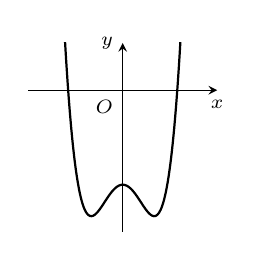
\begin{tikzpicture}[>=stealth,x=1cm,y=1cm,scale=0.4]
			\def\a{1} % Hệ số a phải khác 0
			\def\b{-2}
			\def\c{-3}
			%	\draw[color=gray,dash pattern=on 1pt off 1pt,xstep=1.0cm,ystep=1.0cm] (-5.2,-5.2) grid (5.2,5.2);
			\draw[->] (-3,0) -- (3,0) node[below] {\scriptsize $x$};
			\draw[->] (0,-4.5) -- (0,1.5) node[left] {\scriptsize $y$};
			\draw (0,0)node[below left]{\scriptsize $O$};
			\clip (-3,-4.5)rectangle(3,1.5);
			\draw[thick,samples=150,smooth,domain=-4:4] plot(\x,{\a*(\x)^4+(\b)*(\x)^2+(\c)});
		\end{tikzpicture}
	\end{center}
	\choice
	{$y=-x^3+3x$}
	{$y=x^3-3x-3$}
	{\True $y=x^4-2x^2-3$}
	{$y=-x^4+2x^2-3$}
	\loigiai{
		Đồ thị hàm số $y=ax^4+bx^2+c$ với hệ số $a>0$, $b<0$. Suy ra $y=x^4-2x^2-3$.
	}
\end{ex}

%%==========Câu 14
\begin{ex}%[Đề thi thử Vted 18 Năm 2023-Nguyễn Thắng]%[2H1Y3-2]
	Thể tích của khối chóp tứ giác có đáy là hình vuông cạnh bằng $2$, chiều cao $h=3$ bằng
	\choice
	{$12$}
	{\True $4$}
	{$6$}
	{$18$}
	\loigiai{
		Diện tích đáy $B=2^2=4$. Thể tích của khối chóp là $V=\dfrac{1}{3}Bh=4$.
	}
\end{ex}

%%==========Câu 15
\begin{ex}%[Đề thi thử Vted 18 Năm 2023-Nguyễn Thắng]%[2D3Y1-1]
	Họ nguyên hàm của hàm số $f(x)=x^3$ là
	\choice
	{$3 x^2+C$}
	{\True $\dfrac{1}{4} x^4+C$}
	{$4 x^4+C$}
	{$\dfrac{1}{2} x^2+C$}
	\loigiai{
		Ta có $\displaystyle\int f(x)\mathrm{d}x=\dfrac{x^4}{4}+C$.
	}
\end{ex}

%%==========Câu 16
\begin{ex}%[Đề thi thử Vted 18 Năm 2023-Nguyễn Thắng]%[1D3Y3-3]
	Cho cấp số cộng $\left(u_n\right)$ biết $u_1=2$, công sai $d=3$. Số hạng thứ tư của cấp số cộng đã cho là
	\choice
	{$u_4=18$}
	{\True $u_4=11$}
	{$u_4=54$}
	{$u_4=9$}
	\loigiai{
		Ta có $u_4=u_1+3d=2+3\cdot3=11$.
	}
\end{ex}

%%==========Câu 17
\begin{ex}%[Đề thi thử Vted 18 Năm 2023-Nguyễn Thắng]%[2D2Y2-1]
	Tập xác định của hàm số $y=(2 x-1)^{\frac{1}{3}}$ là
	\choice
	{$\left(-\infty;\dfrac{1}{2}\right)$}
	{$(-\infty ;+\infty)$}
	{$\left[\dfrac{1}{2} ;+\infty\right)$}
	{\True $\left(\dfrac{1}{2} ;+\infty\right)$}
	\loigiai{
		Hàm số xác định khi $2x-1>0\Leftrightarrow x>\dfrac{1}{2}$. Vậy tập xác định của hàm số $\mathscr{D}=\left(\dfrac{1}{2} ;+\infty\right)$.
	}
\end{ex}

%%==========Câu 18
\begin{ex}%[Đề thi thử Vted 18 Năm 2023-Nguyễn Thắng]%[2D1B2-2]
	Cho hàm số $y=f(x)$ có đồ thị như hình vẽ dưới đây
	\begin{center}
		% Đồ thị hàm y=ax^3+bx^2+cx+d. Nếu hệ số lớn cần điều chỉnh hệ trục, vùng lưới, domain và lệnh \clip
		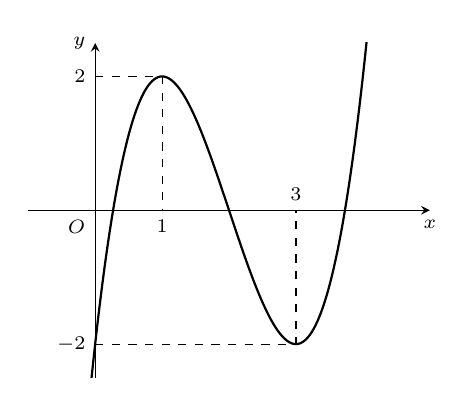
\begin{tikzpicture}[>=stealth,x=1cm,y=1cm,scale=.85]
			\def\a{1} % Hệ số a phải khác 0
			\def\b{-3}
			\def\c{0}
			\def\d{2}
			%	\draw[color=gray,dash pattern=on 1pt off 1pt,xstep=1.0cm,ystep=1.0cm] (-5.2,-5.2) grid (5.2,5.2);
			\draw[->] (-1,0) -- (5,0)node[below]{\scriptsize $x$};
			\draw[->] (0,-2.5) -- (0,2.5) node[left] {\scriptsize $y$};
			\draw[dashed] (0,0)node[below left]{\scriptsize $O$}
			(0,-2)node[left]{\scriptsize $-2$}-|(3,0)node[above]{\scriptsize $3$}
			(0,2)node[left]{\scriptsize $2$}-|(1,0)node[below]{\scriptsize $1$}
			;
			\clip (-1,-2.5)rectangle(5,2.5);
			\draw[thick,samples=150,smooth,domain=-1:5] plot(\x,{\a*(\x-1)^3+(\b)*(\x-1)^2+(\c)*(\x-1)+(\d)});
		\end{tikzpicture}
	\end{center}
	Hàm số đã cho đạt cực đại tại
	\choice
	{\True $x=1$}
	{$x=3$}
	{$x=2$}
	{$x=-2$}
	\loigiai{
		Dựa vào đồ thị, hàm số đã cho đạt cực đại tại $x=1$.
	}
\end{ex}

%%==========Câu 19
\begin{ex}%[Đề thi thử Vted 18 Năm 2023-Nguyễn Thắng]%[2D2Y3-1]
	Với $a$ là số thực dương khác $1$ tùy ý, $\log _a \sqrt{a}$ bằng
	\choice
	{\True $\dfrac{1}{2}$}
	{$-\dfrac{1}{2}$}
	{$-2$}
	{$2$}
	\loigiai{
		Ta có $\log_a\sqrt{a}=\log_aa^\frac{1}{2}=\dfrac{1}{2}\log_aa=\dfrac{1}{2}$.
	}
\end{ex}

%%==========Câu 20
\begin{ex}%[Đề thi thử Vted 18 Năm 2023-Nguyễn Thắng]%[2H3Y3-3]
	Trong KG $Oxyz$, đường thẳng $d\colon \dfrac{x}{3}=\dfrac{y-1}{2}=\dfrac{z+2}{1}$ đi qua điểm nào dưới đây?
	\choice
	{$M(0 ;-1 ;-2)$}
	{$P(3 ; 2 ; 1)$}
	{\True $N(0 ; 1 ;-2)$}
	{$Q(0 ; 1 ; 2)$}
	\loigiai{
		Tọa độ điểm $N(0;1;-2)$ thỏa mãn PTĐT $d$ nên $d$ đi qua $N$.
	}
\end{ex}
%%==========Câu 21
\begin{ex}%[2H3Y2-2]%[BCTuan, dự án tex đề VTED 2023]
	Trong KG $Oxyz$, mặt phẳng vuông góc với đường thẳng $d\colon \heva{&x=1-2t \\& y=2+t \\& z=3+4t}$ có một véc-tơ pháp tuyến là
	\choice
	{$\overrightarrow{n}_3=(2;1;4)$}
	{$\overrightarrow{n}_2=(1;2;-3)$}
	{\True $\overrightarrow{n}_4=(-2;1;4)$}
	{$\overrightarrow{n}_1=(1;2;3)$}
	\loigiai{
		Mặt phẳng  vuông góc với đường thẳng $d\colon \heva{&x=1-2t \\& y=2+t \\& z=3+4t}$ có một véc-tơ pháp tuyến là $\overrightarrow{n}_4=(-2;1;4)$.
	}
\end{ex}
\begin{ex}%[2H3B3-1]%[BCTuan, dự án tex đề VTED 2023]
	Trong KG $Oxyz$, đường thẳng đi qua hai điểm $A(3;-2;4)$ và $B(1;1;2)$ có một véc-tơ chỉ phương là
	\choice
	{$\overrightarrow{u}_2=(4;-1;6)$}
	{\True $\overrightarrow{u}_1=(2;-3;2)$}
	{$\overrightarrow{u}_3=(-2;3;2)$}
	{$\overrightarrow{u}_4=\left(2;-\dfrac{1}{2};3\right)$}
	\loigiai{
		Ta có $\overrightarrow{AB}=(-2;3;-2)=-\overrightarrow{u}_1$ với $\overrightarrow{u}_1=(2;-3;2)$.\\
		Vậy $\overrightarrow{u}_1=(2;-3;2)$ là một véc-tơ chỉ phương của đường thẳng trên.
	}
\end{ex}

%%==========Câu 23
\begin{ex}%[2D1Y4-1]%[BCTuan, dự án tex đề VTED 2023]
	Tiệm cận đứng của đồ thị hàm số $y=\dfrac{4}{x+2}$ là
	\choice{$x=2$}{\True $x=-2$}{$y=0$}{$y=2$}
	\loigiai{
		Tập xác định $\mathscr{D}=\mathbb{R}\setminus \{-2\}$.\\
		Ta có $\lim\limits_{x\to (-2)^+}y=+\infty$ nên $x=-2$ là đường tiệm cận đứng của đồ thị hàm số.
	}
\end{ex}

%%==========Câu 24
\begin{ex}%[2H2Y1-2]%[BCTuan, dự án tex đề VTED 2023]
	Diện tích xung quanh của hình nón có đường sinh $\ell=5$, bán kính đáy $r=3$ bằng
	\choice
	{$30 \pi$}
	{\True $15 \pi$}
	{$48 \pi$}
	{$24 \pi$}
	\loigiai{
		Ta có $S_{\text{xq}}=\pi r\ell =15\pi$.
	}
\end{ex}

%%==========Câu 25
\begin{ex}%[2D2Y4-1]%[BCTuan, dự án tex đề VTED 2023]
	Hàm số nào dưới đây có tập xác định là $\mathbb{R} \setminus \{0\}$?
	\choice
	{$y=3^x$}
	{$y=x^{\tfrac{1}{3}}$}
	{\True $y=x^{-3}$}
	{$y=\log _3 x$}
	\loigiai{
		Hàm số $y=x^{-3}$ có số mũ $-3$ nguyên âm nên điều kiện là $x\ne 0$.
	}
\end{ex}

%%==========Câu 26
\begin{ex}%[1D2Y2-1]%[BCTuan, dự án tex đề VTED 2023]
	Một tổ hợp chập $2$ của tập $S=\{1;2;3;4;5\}$ là
	\choice
	{$\mathrm{C}_5^2$}
	{$\mathrm{A}_5^2$}
	{\True $\{1;2\}$}
	{$(1;2)$}
	\loigiai{
		Một tổ hợp chập $2$ của tập $S=\{1;2;3;4;5\}$ là $\{1;2\}$.
	}
\end{ex}

%%==========Câu 27
\begin{ex}%[2H3Y1-1]%[BCTuan, dự án tex đề VTED 2023]
	Trong KG $Oxyz$, toạ độ của véc-tơ $\overrightarrow{a}=2 \overrightarrow{i}+3 \overrightarrow{k}-\overrightarrow{j}$ là
	\choice
	{$(2;3;-1)$}
	{$(-1;3;2)$}
	{\True $(2;-1;3)$}
	{$(-1;2;3)$}
	\loigiai{
		Ta có $\overrightarrow{a}=2\overrightarrow{i}+3 \overrightarrow{k}-\overrightarrow{j}=2\overrightarrow{i}-\overrightarrow{j}+3 \overrightarrow{k}$ nên $\overrightarrow{a}=(2;-1;3)$.
	}
\end{ex}

%%==========Câu 28
\begin{ex}%[2D3Y2-1]%[BCTuan, dự án tex đề VTED 2023]
	Cho $\displaystyle\int\limits_0^2 f(x) \mathrm{\,d}x=-6$ và $\displaystyle\int\limits_0^4 f(x)\mathrm{\,d}x=3$, khi đó $\displaystyle\int\limits_2^4 f(x)\mathrm{\,d}x$ bằng
	\choice
	{$-9$}
	{$3$}
	{\True $9$}
	{$-3$}
	\loigiai{
		Ta có $\displaystyle\int\limits_2^4 f(x)\mathrm{\,d}x=\displaystyle\int\limits_0^4 f(x)\mathrm{\,d}x-\displaystyle\int\limits_0^2 f(x) \mathrm{\,d}x=3-(-6)=9$.
	}
\end{ex}

%%==========Câu 29
\begin{ex}%[2D1B3-1]%[BCTuan, dự án tex đề VTED 2023]
	Trên đoạn $[-2;1]$, hàm số $y=x^3+3x^2-1$ đạt giá trị nhỏ nhất tại điểm
	\choice
	{$x=-2$}
	{$x=1$}
	{\True $x=0$}
	{$x=-1$}
	\loigiai{
		Hàm số đã cho liên tục trên đoạn $[-2;1]$.\\
		Ta có $y'=3x^2+6x, y'=0\Leftrightarrow \hoac{& x=0\in (-2;1) \\ & x=-2\notin (-2;1).}$\\
		Ta có $y(-2)=3$, $y(0)=-1$, $y(1)=2$.\\
		Vậy $\min\limits_{[-2;1]} y=y(0)=-1$.
	}
\end{ex}
%%==========Câu 30
\begin{ex}%[Nguyễn Văn Sang-Dự Án Đề VTed-2023-Đề 18]%[1D2K5-2]
	Gọi $S$ là tập tất cả các số tự nhiên gồm hai chữ số được lập từ các chữ số $1,2,3,4,5,6$. Chọn ngẫu nhiên một số thuộc $S$, xác suất để số được chọn gồm hai chữ số phân biệt bằng
	\choice
	{\True $\dfrac{5}{6}$}
	{$\dfrac{1}{2}$}
	{$\dfrac{1}{6}$}
	{$\dfrac{5}{12}$}
	\loigiai{
		Số tự nhiên có hai chữ số được lập từ các chữ số $1,2,3,4,5,6$ có $6\cdot6=36$ số.\\
		Số tự nhiên có hai chữ số khác nhau được lập từ các chữ số $1,2,3,4,5,6$ có $6\cdot5=30$ số.\\
		Gọi $A$ là biến cố: \lq\lq  Chọn được số có hai chữ số phân biệt\rq\rq.\\
		Xác suất biến cố $A$ là 
		$$\mathrm{P}(A)=\dfrac{n(A)}{n(\Omega)}=\dfrac{30}{36}=\dfrac{5}{6}.$$
		
	}
\end{ex}

%%==========Câu 31
\begin{ex}%[Nguyễn Văn Sang-Dự Án Đề VTed-2023-Đề 18]%[1H3B3-2]
	\immini
	{
		Cho hình lăng trụ $ABC.A'B'C'$ có tất cả các cạnh bằng nhau. Hình chiếu vuông góc của $A$ trên mặt phẳng $(A'B'C')$ là trung điểm $H$ của $B'C'$ (tham khảo hình bên). Góc giữa hai đường thẳng $AA'$ và $B'C'$ bằng
		\choice
		{$60^{\circ}$}
		{$45^{\circ}$}
		{$30^{\circ}$}
		{\True $90^{\circ}$}
	}
	{
		\begin{tikzpicture}[scale=0.7,yscale=0.7, >=stealth]
			\path 
			(0,0) coordinate (A')
			(2,-2) coordinate (B')
			(4,-1) coordinate (H)
			(6,0) coordinate (C')
			(4,6) coordinate (A)
			(6,4) coordinate (B)
			(10,6) coordinate (C)
			;
			\draw 
			(A')--(B')--(C')
			(A)--(B)--(C)--cycle
			(A)--(A')
			(B)--(B')
			(C)--(C')
			;
			\draw[dashed]
			(A)--(H)
			(A')--(C')
			;
			\foreach \x/\g in {A/90, B/90, C/0, A'/180, B'/-90, C'/0, H/-90}\fill[blue] (\x) circle (1pt)  ($(\x)+(\g:4mm)$) node {$\x$};
		\end{tikzpicture}
	}
	\loigiai{
		\immini
		{
			Ta có $\heva{& B'C'\perp AH \\ & B'C'\perp A'H}\Rightarrow B'C'\perp(A'H'A)$.\\
			Suy ra $B'C'\perp A'A$ hay góc giữa hai đường thẳng $AA'$ và $B'C'$ bằng $90^\circ$.\\
		}
		{
			\begin{tikzpicture}[scale=0.7,yscale=0.7, >=stealth]
				\path 
				(0,0) coordinate (A')
				(2,-2) coordinate (B')
				(4,-1) coordinate (H)
				(6,0) coordinate (C')
				(4,6) coordinate (A)
				(6,4) coordinate (B)
				(10,6) coordinate (C)
				;
				\draw 
				(A')--(B')--(C')
				(A)--(B)--(C)--cycle
				(A)--(A')
				(B)--(B')
				(C)--(C')
				;
				\draw[dashed]
				(A)--(H)--(A')
				(A')--(C')
				;
				\foreach \x/\g in {A/90, B/90, C/0, A'/180, B'/-90, C'/0, H/-90}\fill[blue] (\x) circle (1pt)  ($(\x)+(\g:4mm)$) node {$\x$};
			\end{tikzpicture}
		}
	}
\end{ex}

%%==========Câu 32
\begin{ex}%[Nguyễn Văn Sang-Dự Án Đề VTed-2023-Đề 18]%[2D3B1-2]
	Cho $F$ là một nguyên hàm của hàm số $f(x)$ trên $\mathbb{R}$, khẳng định nào dưới đây đúng?
	\choice
	{$\displaystyle\int \mathrm{e}^x \cdot f(2 \mathrm{e}^x-1) \mathrm{\,d}x=F(2 \mathrm{e}^x-1)+C$}
	{ $\displaystyle\int \mathrm{e}^x \cdot f(2\mathrm{e}^x-1)\mathrm{\,d}x=2 F(2 \mathrm{e}^x-1)+C$}
	{\True $\displaystyle\int \mathrm{e}^x \cdot f(2 \mathrm{e}^x-1)\mathrm{\,d}x=\dfrac{1}{2} F(2 \mathrm{e}^x-1)+C$}
	{ $\displaystyle\int \mathrm{e}^x \cdot f(2 \mathrm{e}^x-1)\mathrm{\,d}x=-\dfrac{1}{2} F(2 \mathrm{e}^x-1)+C$}
	\loigiai{
		Xét $I=\displaystyle\int \mathrm{e}^x \cdot f(2 \mathrm{e}^x-1) \mathrm{\,d}x$.\\
		Đặt $t=2\mathrm{e}^x-1\Rightarrow \mathrm{\,d}t=2\mathrm{e}^x\mathrm{\,d}x$.\\
		Thay vào $I$ ta được  $I=\displaystyle\int \dfrac{1}{2}f(t) \mathrm{\,d}t=\dfrac{1}{2}F(t)+C=\dfrac{1}{2} F(2\mathrm{e}^x-1)+C$.\\
	}
\end{ex}

%%==========Câu 33
\begin{ex}%[Nguyễn Văn Sang-Dự Án Đề VTed-2023-Đề 18]%[2D1B1-1]
	Cho hàm số $f(x)$ có đạo hàm $f'(x)=x^2(x+2), \forall x \in \mathbb{R}$. Hàm số đã cho nghịch biến trên khoảng nào dưới đây?
	\choice
	{$(-2 ; 0)$}
	{$(0 ;+\infty)$}
	{\True $(-\infty ;-2)$}
	{$(-2 ;+\infty)$}
	\loigiai{
		Với hàm số $f(x)$ có đạo hàm $f'(x)=x^2(x+2),\forall x \in \mathbb{R}$.\\
		Xét $f'(x)\leq 0\Leftrightarrow x^2(x+2)\leq 0\Leftrightarrow \hoac{& x=0 \\ & x\leq -2.}$\\
		Vậy hàm số $f(x)$ nghịch biến trên khoảng $(-\infty ;-2)$.	
	}
\end{ex}

%%==========Câu 34
\begin{ex}%[Nguyễn Văn Sang-Dự Án Đề VTed-2023-Đề 18]%[2D3Y3-1]
	Diện tích phần tô đậm trong hình vẽ được giới hạn bởi đồ thị của hai hàm số $y=\dfrac{1}{3} x^2-\dfrac{2}{3} x-\dfrac{2}{3}, y=\sqrt{x}$ và đường thẳng $x=1$ được tính bởi công thức
	\begin{center}
		\begin{tikzpicture}[>=stealth]
			\def\a{1/3}
			\def\b{-2/3}
			\def\c{-2/3}
			\def\f(#1){\a*((#1)^2)+\b*(#1)+\c}
			\def\g(#1){sqrt(#1)}
			\pgfmathsetmacro\ct{-\b/(2*\a)}
			\def\xmin{-2}
			\def\xmax{4.5}
			\def\ymin{-1.}
			\def\ymax{4}
			\fill[gray,smooth] plot[domain=1:4] (\x,{\f(\x)})--plot[domain=4:1] (\x,{\g(\x)})--cycle;
			\draw[->] (\xmin-1,0)--(\xmax+0,0) node[below] { $x$};
			\draw[->] (0,\ymin-1)--(0,\ymax+0) node[left] { $y$};
			\draw (0,0) node [above left] { $O$};
			\draw[thick,smooth,samples=200] plot[domain=\xmin:\xmax] (\x,{\f(\x)});
			\draw[dashed] (\ct,0)--(\ct,{\f(\ct)})
			(1,1) --(1,0)
			(4,0)|-(0,2)
			;
			\fill (\ct,{\f(\ct)}) circle (1pt)
			(1,1) circle (1pt)
			(4,2) circle (1pt)
			;
			\draw (\xmax,{\f(\xmax)}) node [above right]{$y=\dfrac{1}{3} x^2-\dfrac{2}{3}{x}-\dfrac{2}{3}$};
			\def\xmin{0}
			\def\xmax{4.5}
			\def\ymin{0}
			\def\ymax{2.3}
			\draw[thick,smooth,samples=200] plot[domain=\xmin:\xmax] (\x,{\g(\x)});
			\draw ($(\xmax,{\f(\xmax)})+(-90:1)$) node [above right]{$y=\sqrt{x}$};
			\path 
			(1,0) node[below left] {$1$}
			(4,0) node[below] {$4$}
			(0,2) node[left] {$2$}
			;
		\end{tikzpicture}
	\end{center}
	\choice
	{$S=\displaystyle\int\limits_1^4\left(\dfrac{1}{3} x^2-\dfrac{2}{3} x-\dfrac{2}{3}-\sqrt{x}\right) \mathrm{d}x$}
	{\True $S=\dfrac{1}{3} \displaystyle\int\limits_1^4\left(3 \sqrt{x}-x^2+2 x+2\right) \mathrm{d}x$}
	{$S=\displaystyle\int\limits_0^4\left(\sqrt{x}-\dfrac{1}{3} x^2+\dfrac{2}{3} x+\dfrac{2}{3}\right) \mathrm{d}x$}
	{$S=\displaystyle\int\limits_0^4\left(\dfrac{1}{3} x^2-\dfrac{2}{3} x-\dfrac{2}{3}-\sqrt{x}\right) \mathrm{d}x$}
	\loigiai{
		Theo hình vẽ ta có diện tích phần tô đậm là 
		$$S=\displaystyle\int\limits_1^4\left(\sqrt{x}-\dfrac{1}{3} x^2+\dfrac{2}{3} x+\dfrac{2}{3}\right) \mathrm{d}x=\dfrac{1}{3} \displaystyle\int\limits_1^4\left(3 \sqrt{x}-x^2+2 x+2\right) \mathrm{d}x.$$
	}
\end{ex}

%%==========Câu 35
\begin{ex}%[Nguyễn Văn Sang-Dự Án Đề VTed-2023-Đề 18]%[2D2Y3-1]
	Cho $a$ và $b$ là hai số thực dương khác $1$ thỏa mãn $\sqrt{a}=\sqrt[3]{b}$. Tính giá trị $\log _a b$.
	\choice
	{$\log _a b=\dfrac{\sqrt[3]{3}}{2}$}
	{$\log _a b=\dfrac{\sqrt[3]{3}}{\sqrt{2}}$}
	{$\log _a b=\dfrac{3}{2}$}
	{\True $\log _a b=\dfrac{2}{3}$}
	\loigiai{
		Ta có $a$ và $b$ là hai số thực dương  thoả $\sqrt{a}=\sqrt[3]{b}\Leftrightarrow b=a^{\tfrac{3}{2}}$.\\
		Ta được $$\log _a b=\log _a a^{\tfrac{3}{2}}=\dfrac{3}{2}.$$
	}
\end{ex}

%%==========Câu 36
\begin{ex}%[Nguyễn Văn Sang-Dự Án Đề VTed-2023-Đề 18]%[2D4Y1-1]
	Cho hai số thực $a, b$ thỏa mãn $a \cdot 2 i+b(3+i)=6+8 i$. Tổng $a+b$ bằng
	\choice
	{\True $5$}
	{$6$}
	{$4$}
	{$7$}
	\loigiai{
		Ta có  $2ai+b(3+i)=6+8 i\Leftrightarrow 3b+(2a+b)i=6+8i$.\\
		Theo định nghĩa hai số phức bằng nhau ta được 
		$$\heva{& 3b=6 \\ & 2a+b=8}\Leftrightarrow\heva{& a=3 \\ & b=2}\Rightarrow a+b=5. $$
		
	}
\end{ex}

%%==========Câu 37
\begin{ex}%[Nguyễn Văn Sang-Dự Án Đề VTed-2023-Đề 18]%[2H3B3-3]
	Trong KG $Oxyz$, hình chiếu vuông góc của điểm $M(1 ; 2 ;-1)$ trên mặt phẳng $(P) \colon x+2 y-3 z+6=0$ là điểm $H(a;b;c)$. Tổng $a+b+c$ bằng
	\choice
	{$-3$}
	{$-4$}
	{$0$}
	{\True $2$}
	\loigiai{
		Gọi $d$ là đường thẳng qua $M$ và vuông góc mặt phẳng $(P)$.\\
		PTTS đường thẳng $d\colon \heva{& x=1+t \\ &y=2+2t,\,  (t\in\mathbb{R}).\\&z=-1-3t}$\\
		Hình chiếu vuông góc của điểm $M$ trên $(P)$ là giao điểm của $d$ và $(P)$.\\
		Thay $d$ vào $(P)$ ta được 
		$$(1+t)+2(2+2t)-3(-1-3t)+6=0\Leftrightarrow 14t+14=0\Leftrightarrow t=-1.$$
		Vậy toạ độ $H(0;0;2)$ hay $a+b+c=2$.
	}
\end{ex}

%%==========Câu 38
\begin{ex}%[Paul Hieu Nguyen-Dự Án Vted 2023 đề 18]%[1H3K5-3]
	Cho hình chóp đều $S.ABCD$ có độ dài cạnh đáy bằng $4$, mặt bên tạo với mặt phẳng đáy góc $30^{\circ}$. Khoảng cách từ điểm $A$ đến mặt phẳng $(SCD)$ bằng
	\choice
	{$2 \sqrt{3}$}
	{$4 \sqrt{3}$}
	{$\dfrac{4 \sqrt{3}}{3}$}
	{\True $2$}
	\loigiai{
		\immini{Gọi $O$ là tâm mặt đáy và $M$ là trung điểm cạnh $CD$.\\
			Khi đó $SM\perp CD$ và $OM\perp CD$.\\
			Do đó góc giữa mặt bên và mặt phẳng đáy là góc $\widehat{SMO}=30^{\circ}$.\\
			Ta có $OM=2$, $SO=OM\cdot\tan 30^{\circ}=\dfrac{2\sqrt{3}}{3}$.\\
			Vì $AC=2OC$ nên $$\mathrm{d}(A,(SCD))=2\mathrm{d}(O,(SCD))=2\cdot\dfrac{SO\cdot OM}{\sqrt{SO^2+OM^2}}=2.$$}
		{\begin{tikzpicture}[>=stealth,line join=round,line cap=round,font=\footnotesize,scale=1]
				\tikzset{declare function={a=2.2;b=1.3;h=1.7;goc=-140;}}
				\coordinate (A) at (0:0);
				\coordinate (D) at (0:a);
				\coordinate (B) at (goc:b);
				\coordinate (C) at ($(B)+(D)-(A)$);
				\coordinate (O) at ($(A)!.5!(C)$);
				\coordinate (M) at ($(C)!.5!(D)$);
				\coordinate (S) at ($(O)+(0,h)$);
				\draw (M)--(S)--(B)--(C)--(D)--(S)--(C);
				\draw[dashed] (B)--(A)--(D)--(B) (M)--(O)--(S)--(A)--(C);
				\foreach \d/\g in {A/140,B/200,C/-60,D/0,S/90,O/-105,M/-45}
				\fill[black](\d) circle (0.6pt)+(\g:.2)node[scale=.85]{$\d$};
			\end{tikzpicture}
		}
	}
\end{ex}

%%==========Câu 39
\begin{ex}%[Paul Hieu Nguyen-Dự Án Vted 2023 đề 18]%[2D2K6-2]
	Có bao nhiêu số nguyên $x$ thoả mãn $\log _2\left(x^2\right)+\log _3\left(x^3\right) \geq \log _2 x \cdot \log _3 x-4$?
	\choice
	{$27$}
	{\True $134$}
	{$26$}
	{$133$}
	\loigiai{
		Điều kiện $x>0$. Khi đó
		\allowdisplaybreaks
		\begin{eqnarray*}
			& &\log _2\left(x^2\right)+\log _3\left(x^3\right) \geq \log _2 x \cdot \log _3 x-4\\
			&\Leftrightarrow& 2\log _2 x+3\log _3 x \geq \log _2 x \cdot \log _3 x-4\\
			&\Leftrightarrow& 2\log _2 x+\dfrac{3\log _2 x}{\log_2 3} \geq \log _2 x \cdot \dfrac{\log _2 x}{\log _2 3}-4\\
			&\Leftrightarrow& \log _2^2 x-\left(2\log_2 3 + 3\right)\log _2 x-4\log_2 3 \le 0\\
			&\Leftrightarrow& -0{,}897\le\log _2 x \le 7{,}067\\
			&\Leftrightarrow& 0{,}536\le x \le 134{,}056.
		\end{eqnarray*}
		Vì $x$ nguyên nên $x\in\{1;2;3;\ldots;134\}$.\\
		Vậy có $134$ số nguyên thỏa bài toán.
	}
\end{ex}

%%==========Câu 40
\begin{ex}%[Paul Hieu Nguyen-Dự Án Vted 2023 đề 18]%[2D3K2-4]
	Cho hàm số $f(x)$ có đạo hàm $f'(x)=\cos x+1$, $\forall x \in \mathbb{R}$ và $\displaystyle\int\limits_0^{\tfrac{\pi}{2}}f(x) \mathrm{\,d} x=\dfrac{\pi^2}{8}+1$. Khi đó $f\left(\dfrac{\pi}{2}\right)$ bằng
	\choice
	{$\dfrac{\pi}{2}$}
	{\True $\dfrac{\pi}{2}+1$}
	{$\dfrac{\pi}{2}-1$}
	{$1$}
	\loigiai{
		Ta có $f'(x)=\cos x+1 \Rightarrow f(x)=\sin x + x + C$.\\
		Khi đó $\displaystyle\int\limits_0^{\tfrac{\pi}{2}}f(x) \mathrm{\,d} x=\displaystyle\int\limits_0^{\tfrac{\pi}{2}} (\sin x+x+C) \mathrm{\,d}x = \left(-\cos x + \dfrac{x^2}{2}+Cx\right)\bigg|_0^{\tfrac{\pi}{2}}=\dfrac{\pi^2}{8}+C\cdot\dfrac{\pi}{2}+1$.\\
		Vì $\displaystyle\int\limits_0^{\tfrac{\pi}{2}}f(x) \mathrm{\,d} x=\dfrac{\pi^2}{8}+1$ nên $\dfrac{\pi^2}{8}+C\cdot\dfrac{\pi}{2}+1=\dfrac{\pi^2}{8}+1 \Rightarrow C=0$.\\
		Do đó $f(x)=\sin x + x$. Vậy $f\left(\dfrac{\pi}{2}\right)=\dfrac{\pi}{2}+1$.
	}
\end{ex}

%%==========Câu 41
\begin{ex}%[Paul Hieu Nguyen-Dự Án Vted 2023 đề 18]%[2H1K3-2]
	Cho khối chóp $S.ABC$ có đáy $ABC$ là tam giác đều, hình chiếu vuông góc của đỉnh $S$ trên mặt phẳng đáy là trung điểm $H$ của cạnh $AB$. Biết $SC=3a$ và góc giữa hai mặt phẳng $(SAC)$ và $(SBC)$ bằng $90^0$. Thể tích khối chóp đã cho bằng
	\choice
	{\True $2 a^3$}
	{$\dfrac{1}{2}a^3$}
	{$4 a^3$}
	{$3 a^3$}
	\loigiai{
		\immini{Đặt $A B=B C=C A=x$, ($x>0$).\\
			Gọi $A K$ là đường cao của tam giác $SAC$. Vì $\triangle SAC = \triangle SBC$ (c-c-c) nên $BK$ cũng là đường cao của tam giác $SBC$.\\
			Ta có $AK\perp SC$, $BK\perp SC \Rightarrow((S A C),(S B C))=\widehat{A K B}=90^0$.\\
			Do đó $K H=\dfrac{A B}{2}=\dfrac{x}{2}$.\\
			Ta có $C H=\dfrac{\sqrt{3}x}{2}\Rightarrow S H=\sqrt{S C^2-C H^2}=\sqrt{9 a^2-\dfrac{3}{4}x^2}$.}
		{
			\begin{tikzpicture}[>=stealth,line join=round,line cap=round,font=\footnotesize,scale=1]
				\tikzset{declare function={a=2.5;b=1.5;h=1.7;goc=-50;}}
				\coordinate (A) at (0,0);
				\coordinate (C) at (a,0);
				\coordinate (B) at (goc:b);
				\coordinate (H) at ($(A)!0.5!(B)$);
				\coordinate (K) at ($(S)!0.4!(C)$);
				\coordinate (S) at ($(H)+(0,h)$);
				\draw (S)--(A)--(B)--(C)--(S)--(B)--(K) (S)--(H);
				\draw[dashed] (K)--(A)--(C)--(H)--(K);
				\foreach \d/\g in {A/180,B/-90,C/0,S/90,H/-120,K/60}
				\fill[black](\d) circle (0.6pt)+(\g:.2)node[scale=.85]{$\d$};
			\end{tikzpicture}
		}
		\noindent
		và $H K=\dfrac{HS\cdot HC}{SC}\Rightarrow \dfrac{\dfrac{\sqrt{3}}{2}x \sqrt{9 a^2-\dfrac{3}{4}x^2}}{3 a}=\dfrac{x}{2}\Rightarrow x=2 \sqrt{2}a \Rightarrow S H=\sqrt{3}a$.\\
		Vậy $V_{S \cdot A B C}=\dfrac{1}{3}S_{A B C}\cdot S H=\dfrac{1}{3}\cdot \dfrac{\sqrt{3}}{4}(2 \sqrt{2}a)^2 \cdot \sqrt{3}=2 a^3$.
	}
\end{ex}

%%==========Câu 42
\begin{ex}%[Paul Hieu Nguyen-Dự Án Vted 2023 đề 18]%[2H3K3-7]
	Trong KG $Oxyz$, cho điểm $E(3 ; 0 ; 5)$ và hai đường thẳng $d_1\colon \dfrac{x-2}{1}=\dfrac{y-2}{1}=\dfrac{z}{-1}$; $d_2\colon \left\{\begin{aligned} &x=2+t \\ &y=-1+2 t \\ &z=-3 t\end{aligned}\right.$. Gọi $(P)$ là mặt phẳng đi qua $E$, cắt hai đường thẳng $d_1$, $d_2$ lần lượt tại các điểm $A$ và $B$ sao cho $A B=\sqrt{6}$. Điểm nào dưới đây thuộc $(P)$?
	\choice
	{\True $M(1 ; 2 ; 3)$}
	{$Q(3 ; 2 ;-1)$}
	{$P(1 ;-2 ; 3)$}
	{$N(2 ;-1 ; 3)$}
	\loigiai{
		Gọi $A(a+2 ; a+2 ;-a) \in d_1$, $B(b+2 ; 2 b-1 ;-3 b) \in d_2$. \\
		Ta có $AB^2=(b-a)^2+(2 b-a-3)^2+(a-3 b)^2=6
		\Leftrightarrow 3 a^2+6 a(1-2 b)+14 b^2-12 b+3=0$. \\
		Phương trình trên có $\Delta_a'=9(1-2 b)^2-3\left(14 b^2-12 b+3\right)=-6 b^2 \leq 0$. \\
		Do vậy để tồn tại $a$ thoả mãn phương trình thì $b=0 \Rightarrow 3 a^2+6 a+3=0 \Leftrightarrow a=-1$.\\
		Khi đó $A(1 ; 1 ; 1)$, $B(2 ;-1 ; 0) \Rightarrow \overrightarrow{n}_P=\left[\overrightarrow{A B}, \overrightarrow{A E}\right]=(-9 ;-6 ; 3)=-3(3 ; 2 ;-1)$. \\
		Vậy $(P)\colon 3 x+2 y-z-4=0$ đi qua điểm $M(1 ; 2 ; 3)$.
	}
\end{ex}

%%==========Câu 43
\begin{ex}%[Paul Hieu Nguyen-Dự Án Vted 2023 đề 18]%[2D4K4-1]
	Trên tập số phức, cho phương trình $z^2+a z+b=0$, ($a$, $b \in \mathbb{R}$). Có bao nhiêu số phức $w$ sao cho phương trình đã cho có hai nghiệm là $z_1=(6-i)w-2i$ và $z_2=(\overline{w}-5+i)|w|$?
	\choice
	{\True $4$}
	{$3$}
	{$6$}
	{$5$}
	\loigiai{
		\textbf{TH1:} Nếu $z_1$, $z_2 \in \mathbb{R}$ thì\\ 
		$z_1=(6-i) w-2 i=(6-i)(x+y i)-2 i$ có phần ảo bằng $0$, suy ra $-x+6 y-2=0$.\\
		$z_2=(\overline{w}-5+i)|w|=\sqrt{x^2+y^2}\left[(x-5)+(1-y) i\right]$ có phần ảo bằng $0$, suy ra $(1-y) \sqrt{x^2+y^2}=0$.\\
		Giải hệ $\left\{\begin{aligned} &-x+6 y-2=0 \\&(1-y)\sqrt{x^2+y^2}=0\end{aligned}\right.$
		ta được $x=4$; $y=1\Rightarrow w=4+i$.\\
		\textbf{TH2:} Nếu $z_1$, $z_2 \notin \mathbb{R}$ thì\\
		$z_1=\overline{z_2}\Leftrightarrow(6-i) w-2 i=(w-5-i)|w|=tw-5t-ti$, ($t=|w|$, ($t \geq 0$)).\\
		$\Leftrightarrow w[(t-6)+i]=5 t+(t-2) i \Rightarrow t\left[(t-6)^2+1\right]=25 t^2+(t-2)^2$\\
		$\Leftrightarrow t(t^2-12t+37)=26t^2-4t+4\Leftrightarrow t^3-38t^2+41t-4=0$\\
		$\Rightarrow t=1$; $t \approx 0{,}11$ ; $t \approx 36{,}89$ tương ứng $3$ số phức $w$.\\
		Vậy có tất cả $4$ số phức $w$ thoả mãn.
	}
\end{ex}

%%==========Câu 44
\begin{ex}%[Paul Hieu Nguyen-Dự Án Vted 2023 đề 18]%[2D1G2-6]
	Cho hàm số $f(x)$ có đạo hàm $f'(x)=6 x^2-6 x-12$, $\forall x\in \mathbb{R}$ và $f(-1)=2$. Số giá trị nguyên của tham số $m$ để hàm số $g(x)=\left|f\left(x^4-2 x^2\right)-m\right|$ có ít nhất $9$ điểm cực trị là
	\choice
	{$27$}
	{$20$}
	{\True $26$}
	{$19$}
	\loigiai{
		Hàm số $f(x)$ có hai điểm cực trị là $x=-1$; $x=2$.\\
		Xét $u(x)=f\left(x^4-2 x^2\right)-m$ có bảng biến thiên như sau:
		\begin{center}
			\begin{tikzpicture}
				\tkzTabInit[nocadre=false,lgt=2.2,espcl=2.8,deltacl=0.6]
				{$x$/0.6,$x^4-2x^2$/0.6,$u(x)$/2.5}
				{$-\infty$, $-1$, $0$, $1$, $+\infty$}
				\tkzTabLine{+\infty,2,-1, ,0, ,-1,2,+\infty}
				\path
				(N12)node[below](A){$+\infty$}
				($(N13)!.5!(N23)$)node[above](B){$-25-m$}
				(N22)node[below](C){$2-m$}
				($(N32)!.5!(N33)$)node(D){$-5-m$}
				(N42)node[below](E){$2-m$}
				($(N43)!.5!(N53)$)node[above](F){$-25-m$}
				(N52)node[below](G){$+\infty$};
				\foreach\x/\y in{A/B,B/C,C/D,D/E,E/F,F/G}\draw[-latex](\x)--(\y);
			\end{tikzpicture}
		\end{center}
		Trong đó 
		$f(2)=2+\displaystyle\int\limits_{-1}^2 6\left(x^2-x-2\right)\mathrm{\,d}x=-25$; $f(0)=2+\displaystyle\int\limits_{-1}^0 6\left(x^2-x-2\right)\mathrm{\,d}x=-5$.\\
		Vậy $g(x)=|u(x)|$ có ít nhất $9$ điểm cực trị khi $u(x)$ có ít nhất $4$ lần đổi dấu
		$$\Leftrightarrow-25-m<0<2-m \Leftrightarrow-25<m<2 \Rightarrow m \in\{-24,-23, \ldots, 1\}.$$
	}
\end{ex}
%%==========Câu 45
\begin{ex}%[2H2G2-5]%[Phạm Hoài, Tex-hoa-VTed-2022-2-23]
	Trong KG $Oxyz$, cho điểm $M(3;0;5)$ và mặt cầu $(S)\colon (x-1)^2+(y+2)^2+(z-4)^2=81$. Xét các điểm $A$, $B$, $C$ di động trên $(S)$ sao cho $MA$, $MB$, $MC$ đôi một vuông góc và gọi $E$ là đỉnh đối diện với đỉnh $M$ của hình hộp chữ nhật có ba cạnh $MA$, $MB$, $MC$. Khoảng cách từ  $E$ đến mặt phẳng $(Oxy)$ có giá trị lớn nhất bằng
	\choice
	{$21$}
	{\True $15$}
	{$17$}
	{$19$}
	\loigiai{
		\begin{itemize}
			\item \textbf{Cách 1:}
			\immini{
				Mặt cầu $(S)$ có tâm $I(1;-2;4)$, $R=9$ và $IM=3$, $IA=IB=IC=R=9$.\\
				Theo tính chất hình hộp ta có \begin{eqnarray*}&&\overrightarrow{ME}=\overrightarrow{MA}+\overrightarrow{MB}+\overrightarrow{MC}\\&\Leftrightarrow & \overrightarrow{IE}-\overrightarrow{IM}=\overrightarrow{IA}-\overrightarrow{IM}+\overrightarrow{IB}-\overrightarrow{IM}+\overrightarrow{IC}-\overrightarrow{IM}\\
					&\Leftrightarrow & \overrightarrow{IE}+2\overrightarrow{IM}=\overrightarrow{IA}+\overrightarrow{IB}+\overrightarrow{IC}
				\end{eqnarray*}
				Bình phương hai vế ta có $$IE^2+4IM^2+4\cdot \overrightarrow{IE}\cdot \overrightarrow{IM}=3R^2+2\left(\overrightarrow{IA}\cdot \overrightarrow{IB}+\overrightarrow{IB}\cdot \overrightarrow{IC}+\overrightarrow{IC}\cdot \overrightarrow{IA}\right).$$}
			{\begin{tikzpicture}[>=stealth,line width=1pt,line join=round,line cap=round,scale=1]
					\path 
					(0,0) coordinate (M)
					(-1,-1.5) coordinate (A)
					(5,0) coordinate (B)
					($(A)+(B)-(M)$) coordinate (E')
					($(M)+(0,2.5)$) coordinate (C)
					($(A)+(0,2.5)$) coordinate (A')
					($(E')+(0,2.5)$) coordinate (E)
					($(B)+(0,2.5)$) coordinate (B')
					;
					\draw (A')--(A)--(E')--(E)--(A')--(C)--(B')--(B)--(E') (E)--(B');
					\draw[dashed] (C)--(A)--(B)--(C)--(M)--(A) (M)--(B);
					\foreach \x/\g in {A/180,A'/180,B/0, B'/90,M/45,E/90,E'/-90,C/90}
					\draw[fill=black] (\x) circle (.03)+(\g:.3) node{$\x$};
					
			\end{tikzpicture}}
			Sử dụng tích vô hướng của hai véctơ chung gốc dạng $$\overrightarrow{OX}\cdot \overrightarrow{OY}=\dfrac{OX^2+OY^2-XY^2}{2}.$$
			Suy ra
			\begin{eqnarray*}&&IE^2+4IM^2+4\cdot \overrightarrow{IE}\cdot \overrightarrow{IM}\\
				&=&3R^2+\left(IA^2+IB^2-AB^2\right)+\left(IB^2+IC^2-BC^2\right)+\left(IC^2+IA^2-CA^2\right)\\
				&\Leftrightarrow & 3IE^2+6IM^2-2EM^2=9R^2-\left(AB^2+BC^2+CA^2\right)\\
				&\Leftrightarrow & IE^2+2IM^2=3R^2+\dfrac{1}{3}\left[2EM^2-\left(AB^2+BC^2+CA^2\right)\right].
			\end{eqnarray*}
			Mặt khác theo tính chất hình hộp chữ nhật thì
			\begin{itemize}
				\item[$\bullet$] $ME^2=MA^2+MB^2+MC^2$.
				\item[$\bullet$] $AB^2+BC^2+CA^2=2\left(MA^2+MB^2+MC^2\right)$.
			\end{itemize} 
			Do đó $IE^2+2IM^2=3R^2\Rightarrow IE=\sqrt{3R^2-2IM^2}=\sqrt{3\cdot 81-2\cdot 9}=15$.\\
			\immini{ Gọi $H$ là hình chiếu của $E$ lên mặt phẳng $(Oxy)$.\\
				$K(1;-2;0)$ là hình chiếu của $I$ lên mặt phẳng $(Oxy)$.\\ \\Khi đó $d(E;(Oxy))=EDH\leq EK\leq IK+IE=d(I;(Oxy))+IE=4+5=19$.\\
				Dấu \lq \lq=\rq \rq\, xảy ra khi và chỉ khi $H\equiv K(1;-2;0)$ và $E$, $I$, $K$ thẳng hàng theo thứ tự. \\
				Hay $\overrightarrow{EI}=\dfrac{EI}{IK}\overrightarrow{IK}=\dfrac{15}{4}\overrightarrow{IK}=\dfrac{15}{4}(0;0;-4)\Rightarrow E(1;-2;19).$ }
			{\begin{tikzpicture}[>=stealth,line width=1pt,line join=round,line cap=round,scale=1]
					\path 
					(0,0) coordinate (O)
					(-1,-1.5) coordinate (A)
					(5,0) coordinate (B)
					($(A)+(B)-(M)$) coordinate (D)
					(1,-0.5) coordinate (K)
					($(K)+(2,0)$) coordinate (H)
					($(K)+(0,1.3)$) coordinate (I)
					($(H)+(0,2.5)$) coordinate (E)
					(1,0) coordinate (T)
					(3,0) coordinate (U)
					;
					\draw (O)--(A)--(D)--(B)(I)--(K)--(H)--(E)--(K) (E)--(I)(O)--(T) (U)--(B);
					\draw[dashed] (T)--(U);
					\foreach \x/\g in {K/-90,H/-90, I/90,E/90}
					\draw[fill=black] (\x) circle (.03)+(\g:.3) node{$\x$};
					\node at ($(A)+(25:1)$){\small $(Oxy)$};
			\end{tikzpicture}}
			\item \textbf{Cách 2:}
			\immini{
				Chọn hệ trục toạ độ mới sao cho $M(0;0;0)$, $A(a;0;0)$, $B(0;b;0)$, $C(0;0;c)\Rightarrow E(a;b;c)$ và  $I(x;y;z)$.\\
				Theo giả thiết $IM=3$, $IA=IB=IC=R=9$. Ta có hệ $\heva{&x^2+y^2+z^2=9\\&(x-a)^2+y^2+z^2=81\\&x^2+(y-b)^2+z^2=81\\&x^2+y^2+(z-c)^2=81.}$\\
				$\Rightarrow IE^2=(x-a)^2+(y-b)^2+(z-c)^2=3\cdot 81-2\cdot 9=225\Rightarrow IE=15.$\\
				Các bước còn lại làm như ở cách 1.}
			{\begin{tikzpicture}[>=stealth,line width=1pt,line join=round,line cap=round,scale=1]
					\draw[->] (0,0)--(0,0)%
					node[above left]{$M$}--(4,0) node[below]{$y$};
					\draw[->] (0,0) --(0,4) node[right]{$z$};
					\draw[->] (0,0) --(-3,-3) node[right]{$x$};
					\draw[dashed] (-2,-2)node[left]{$A$}--(1,-2)--(3,0)node[above]{$B$} (1,-2)--(1,1)node[right]{$E$}--(0,3)node[right]{$C$} ;
			\end{tikzpicture}}
		\end{itemize}
	}
\end{ex}

%%==========Câu 46
\begin{ex}%[2D1G5-4]%[Phạm Hoài, Tex-hoa-VTed-2022-2-23]
	\immini{Cho hàm số bậc bốn $f(x)$ có đồ thị $(C)$ như hình vẽ. Đường thẳng $d\colon y=g(x)$ là tiếp tuyến của $(C) $ tại điểm có hoành độ $x=3$. Số nghiệm thực phân biệt của phương trình $\dfrac{f(x)-4}{g(x)-4}=\dfrac{g(x)}{f(x)}$ là
		\choice
		{$7$}
		{\True $4$}
		{$5$}
		{$6$}}
	{\begin{tikzpicture}[>=stealth,x=1cm,y=1cm]
			\draw[->] (-2,0)--(0,0)%
			node[below right]{$O$}--(4,0) node[below]{$x$};
			\draw[->] (0,-1) --(0,5) node[right]{$y$};
			\draw (-2,4)..controls (-1,-1) and (-0.5,-1)..(0,0)..controls (1,3) and (1.5,3)..(3,0)..controls (3.2,-.5) and (3.6,-.5)..(4,4);
			\draw[dashed] (1.35,0)node[below]{$c$}--(1.35,2.25)--(0,2.25)node[left]{$2$} (-1,0)node[below]{$a$}(3,0)node[below]{$3$}  (3.7,0)node[below]{$b$}(0,4.1)node[left]{$4$}(4,4)node[above]{$(C)$} ;
			
			\path (3,0)coordinate (m)
			(1.35,2.25)coordinate (n)
			($(n)!1!180:(m)$) coordinate (d)
			($(m)!0.5!180:(n)$) coordinate (x);
			\draw (x)--(d);
			\foreach \x/\g in {d/90}
			\draw[fill=black] (\x) circle (0)+(\g:.3) node{$\x$};
	\end{tikzpicture}}
	\loigiai{
		Điều kiện $\heva{&f(x)\neq 0\\&g(x)-4\neq 0}\Leftrightarrow \heva{&x\notin \{a;0;3;b\}\\&x\neq 0}\Leftrightarrow x\notin \{a;0;3;b\}$ trong đó $a$, $b$ là các hoành độ giao điểm của $(C)$ và trục hoành như hình vẽ
		\begin{center}
			\begin{tikzpicture}[>=stealth,x=1cm,y=1cm]
				\draw[->] (-2,0)--(0,0)%
				node[below right]{$O$}--(4,0) node[below]{$x$};
				\draw[->] (0,-1) --(0,5) node[right]{$y$};
				\draw (-2,4)..controls (-1,-1) and (-0.5,-1)..(0,0)..controls (1,3) and (1.5,3)..(3,0)..controls (3.2,-.5) and (3.6,-.5)..(4,4);
				\draw[dashed] (1.35,0)node[below]{$c$}--(1.35,2.25)--(0,2.25)node[left]{$2$} (-1,0)node[below]{$a$}(3,0)node[below]{$3$}  (3.7,0)node[below]{$b$}(0,4.1)node[left]{$4$}(4,4)node[above]{$(C)$} ;
				
				\path (0,0)coordinate (O)
				(3,0)coordinate (m)
				(1.35,2.25)coordinate (n)
				($(n)!1!180:(m)$) coordinate (d)
				($(m)!0.5!180:(n)$) coordinate (x)
				($(O)!0.5!180:(n)$) coordinate (d')
				($(n)!0.5!180:(O)$) coordinate (x')
				;
				\draw (x)--(d) (x')--(d');
				\foreach \x/\g in {d/90}
				\draw[fill=black] (\x) circle (0)+(\g:.3) node{$\x$};
				\node at ($(d')+(-90:0.4)$){\small $y=4-g(x)$};
			\end{tikzpicture}
		\end{center}
		Đặt $a=f(x)$; $b=g(x)\Rightarrow \dfrac{a-4}{b-4}=\dfrac{b}{a}\Leftrightarrow \hoac{&a=b\\&a=4-b}\Leftrightarrow \hoac{&f(x)=g(x)\\&f(x)=4-g(x).}$\\
		Đường thẳng $y=g(x)$ cắt $(C)$ tại $3$ điểm phân biệt trong đó hai điểm có hoành độ là $x=c$, $x=3$.\\
		Đường thẳng $y=4-g(x)$ qua hai điểm $(0;0)$, $(c;2)$ cắt $(C)$ tại bốn điểm phân biệt trong đó có hai điểm có hoành độ là $x=0$, $x=c$.\\
		Đối chiếu với điều kiện suy ra phương trình có tất cả $(3+4)-2-1=4$ nghiệm. 
	}
\end{ex}

%%==========Câu 47
\begin{ex}%[2D4G5-2]%[Phạm Hoài, Tex-hoa-VTed-2022-2-23]
	Xét hai số phức $z_1$, $z_2$ thoả mãn $\mid z_1-2z_2=4\mid $ và $\mid 3z_1+z_2\mid =5$. Gọi $M$, $m$ lần lượt là giá trị lớn nhất và giá trị nhỏ nhất của biểu thức $P=
	\mid 5z_1-3z_2\mid +\mid z_1+5z_2 \mid $, khi đó $M^2-m^2$ bằng
	\choice
	{$325$}
	{$125$}
	{$247$}
	{\True $100$}
	\loigiai{
		Đặt $a=z_1-2z_2$, $b=3z_1+z_2\Rightarrow \heva{&5z_1-3z_2=2a+b\\&z_1+5z_2=b-2a\\&|a|=4\\&|b|=5.}$\\
		Khi đó $P=\mid 2a+b\mid +\mid b-2a\mid $.\\ Gọi $A$, $B$ là điểm biểu diễn hai số phức $a$ và $b$.\\
		Khi đó $\mid a\mid =\mid \overrightarrow{OA}\mid =4; \mid b\mid =\mid \overrightarrow{OB}\mid =5$ và 
		$$\mid 2a+b\mid ^2=\left(2\overrightarrow{OA}+\overrightarrow{OB}\right)^2=4\overrightarrow{OA}^2+\overrightarrow{OB}+4\overrightarrow{OA}\overrightarrow{OB}=64+25+4OA\cdot OB\cos (\overrightarrow{OA},\overrightarrow{OB})=89+80x$$
		$$\mid b-2a\mid ^2=\left(-2\overrightarrow{OA}+\overrightarrow{OB}\right)^2=4\overrightarrow{OA}^2+\overrightarrow{OB}-4\overrightarrow{OA}\overrightarrow{OB}=64+25-4OA\cdot OB\cos (\overrightarrow{OA},\overrightarrow{OB})=89-80x$$
		Trong đó $x=\cos (\overrightarrow{OA},\overrightarrow{OB})\in [-1;1]$.\\
		Vậy $P=g(x)=\sqrt{89+80x}+\sqrt{89-80x}$.\\\\
		Tập xác định $\mathscr{D}=[-1;1]$.
		$g'(x)=\dfrac{80}{2\sqrt{89+80x}}-\dfrac{80}{\sqrt{89-80x}}$.\\
		$g'(x)=0\Leftrightarrow \sqrt{89-80x}-\sqrt{89+90x}=0\Leftrightarrow x=0$.\\
		Bảng xét dấu
		\begin{center}
			\begin{tikzpicture}
				\foreach \x/\texn in {-4/x,
					-3/-\infty,-1/-1, 2/0,5/1,7/+\infty } \path
				(\x,3.5)node{$\texn$};
				\foreach \x/\texn in
				{-4/f'(x),,0.5/+,2/0,4.5/-,} \path
				(\x,2.5)node{$\texn$};
				\foreach \x/\y/\texn in {-4/1/f(x),
					-0.7/-1.3/16,2/1.8/2\sqrt{89},4.7/-1.3/16}
				\path (\x,\y) node(\x){$\texn$};
				\draw[-stealth] (-0.7,-1.2)--(1.7,1.55);
				\draw[-stealth](2.3,1.55)--(4.7,-1.2);
				\draw
				(-4.5,4)--(7.5,4) (-3.5,4)--(-3.5,-1.5)
				(-4.5,3)--(7.5,3) (-4.5,2)--(7.5,2)(-1,3)--(-1,-1.5)(5.1,3)--(5.1,-1.5)
				(-4.5,4) rectangle (7.5,-1.5);
				\begin{scope}
					\clip (-3.5,-1.5) rectangle (-1,4);
					\fill[pattern=north east lines] (-3.5,4)--(-3.5,-1.5)--(-1,-1.5)--(-1,4)--cycle;
					
				\end{scope}
				\begin{scope}
					\clip (5,-1.5) rectangle (7.5,4);
					\fill[pattern=north east lines] (5.1,4)--(5.1,-1.5)--(7.5,-1.5)--(7.5,4)--cycle;
					
				\end{scope}
				
			\end{tikzpicture}
		\end{center}	
		$\Rightarrow M=\max \limits_{[-1;1]} g(x)=g(0)=2\sqrt{89}$.\\
		$m=\min \limits_{[-1;1]} g(x)=g(\pm 1)=16$.\\
		$\Rightarrow M^2-m^2=\left(2\sqrt{89}\right)^2-16^2=100$.
	}
\end{ex}

%%==========Câu 48
\begin{ex}%[2H2G1-5]%[Phạm Hoài, Tex-hoa-VTed-2022-2-23]
	Cho hình trụ có bán kính đáy và chiều cao cùng bằng $2a$ và hai đường tròn đáy tâm $O$ và $O'$. Xét hai điểm $A$, $B$ lần lượt di động trên đường tròn  tâm $O$ và đường tròn đáy tâm $O'$ sao cho $AB$ tạo với $OO'$ góc $\alpha$ ($0<\alpha <90^{\circ}$). Khi thể tích khối tứ diện $OAO'B$ đạt giá trị lớn nhất thì $\tan \alpha$ bằng
	\choice
	{\True $\sqrt{2}$}
	{$\dfrac{1}{\sqrt{2}}$}
	{$\sqrt{\dfrac{2}{3}}$}
	{$\dfrac{1}{\sqrt{3}}$}
	\loigiai{
		\immini{Ta có $r=h=2a$. Hạ đường sinh $AA'$.\\
			Khi đó $OO'\parallel AA'\Rightarrow \alpha =\widehat{(AB, OO')}=\widehat{(AB, AA')}=\widehat{A'AB}.$\\
			Kẻ $BH\perp O'A'\Rightarrow BH\perp (OAO')$.\\
			Ta có \begin{eqnarray*}
				V_{OAO'B'}&=&\dfrac{1}{3}S_{\triangle OAO'}\cdot d(B,(OAO'))\\
				&=&\dfrac{1}{3}\cdot \dfrac{1}{2}\cdot OA\cdot OO'\cdot BH=\dfrac{2a^2}{3}\cdot BH.
		\end{eqnarray*}}
		{\begin{tikzpicture}
				\path 
				(0,0) coordinate (O')
				(180:2 and 0.7) coordinate (A')
				(0:2 and 0.7) coordinate (D)
				(-60:2 and 0.7) coordinate (B)
				($(O')!(B)!(D)$) coordinate (H) 
				($(O')+(0,-3.5)$) coordinate (O)
				($(A')+(0,-3.5)$) coordinate (A)
				($(D)+(0,-3.5)$) coordinate (D');
				\draw 
				(A') arc (-180:0:2 and 0.7)
				(A') arc (180:0:2 and 0.7)
				(A) arc (-180:0:2 and 0.7)
				(A')--(D)--(B)--(A')(O')--(B)--(H) (A')--(A) (D)--(D')
				;
				\draw[dashed]
				(B)--(O)--(O')--(A)--(D') (A)--(B)
				(A) arc (180:0:2 and 0.7)
				;
				\foreach \x/\g in {A/180,A'/180,O/-90, O'/90,H/90,B/-70,D/0}
				\draw[fill=black] (\x) circle (.03)+(\g:.3) node{$\x$};
				\pic[draw, angle radius =1.5mm, angle eccentricity=1.5] {right angle = B--H--D};
		\end{tikzpicture}}
		\immini{Do đó thể tích khối tứ diện $OAO'B$ đạt giá trị lớn nhất khi và chỉ khi $BH_{\max}$.\\
			Ta có $BH\leq BO'=r=2a$. \\
			Dấu \lq\lq =\rq\rq\,  xảy ra khi $H\equiv O'\Rightarrow \triangle ABD$ vuông cân tại $B$.\\
			Suy ra $A'B=\sqrt{2}r=2\sqrt{2}a$.\\
			Xét $\triangle A'AB$ có $\tan \alpha =\dfrac{A'B}{AA'}=\dfrac{2\sqrt{2}a}{2a}=\sqrt{2}.$ }
		{\begin{tikzpicture}
				\def \r{2}
				\path 
				(0,0) coordinate (O')
				(180:\r) coordinate (A')
				(0:\r) coordinate (D)
				(120:\r) coordinate (B)
				($(O')!(B)!(D)$) coordinate (H) 
				;
				\draw 
				(O') circle (\r ) (A')--(B)--(D)--(A') (O')--(B)--(H)
				;
				
				\foreach \x/\g in {A'/180, O'/-90,H/-90,B/90,D/0}
				\draw[fill=black] (\x) circle (.03)+(\g:.3) node{$\x$};
				\pic[draw, angle radius =1.5mm, angle eccentricity=1.5] {right angle = B--H--A'};
		\end{tikzpicture}}
	}
\end{ex}

%%==========Câu 49
\begin{ex}%[2D2G6-5]%[Phạm Hoài, Tex-hoa-VTed-2022-2-23]
	Có bao nhiêu số nguyên $a\in [-30;30]$ sao cho ứng với mỗi $a$  có không quá $5$ số nguyên $x$ thoả mãn $4^{x-13}+4^{x+1-13}\leq \log_3(1+x)-\log_3(x+a+1)$? 
	\choice
	{$23$}
	{$53$}
	{$22$}
	{\True $54$}
	\loigiai{
		\begin{itemize}
			\item \textbf{Trường hợp 1.}
			Nếu $a\geq 0\Rightarrow $ VP $\leq 0$, VT $>0$. Do đó $S_x=\varnothing$ không chứa số nguyên nào nên thoả mãn.
			\item \textbf{Trường hợp 2.} Nếu $a<0$ điều kiện của bất phương trình $
			\heva{&x>-1\\&x<-a-1}\Leftrightarrow x>-a-1.$\\
			Bất phương trình tương đương $g(x)=4^{x-13}+4^{a+x-13}-\log_3(1+x)+\log_3(a+x+1)\leq 0$.\\
			Ta có  \begin{eqnarray*} g'(x)&=&4^{x-3}\ln 4+4^{x+a-13}\ln 4-\dfrac{1}{(x+1)\ln 3}+\dfrac{1}{(x+a+1)\ln 3}\\
				&=&4^{x-13}\ln 4+4^{x+1-13}\ln 4-\dfrac{1}{\ln 3}\cdot \dfrac{a}{(x+1)(x+a+1)}>0,
			\end{eqnarray*} $\forall a<0$, $\forall x>-a-1$
			\\ Bảng biến thiên
			\begin{center}
				\begin{tikzpicture}
					\foreach \x/\texn in {-4/x,
						-2.5/-a-1,0/x_0, 3/-a+5,6/+\infty} \path
					(\x,3.5)node{$\texn$};
					\foreach \x/\y/\texn in {-4/1/g(x),
						-3/-1/-\infty,6/1.5/+\infty}
					\path (\x,\y) node(\x){$\texn$};
					\draw[-stealth] (-3)--(6);
					\draw
					(-4.5,4)--(6.5,4) (-3.5,4)--(-3.5,-1.5)
					(-4.5,3)--(6.5,3) (-2,-0.2)--(5,-0.2)
					(-4.5,4) rectangle (6.5,-1.5);
					\draw[dashed] (0,3)--(0,-0.2)(3,3)--(3,0.7);
					\node at ($(5,-0.2)+(90:0.4)$){\small $y=0$};
				\end{tikzpicture}
			\end{center}
			Suy ra tập nghiệm của bất phương trình là $S_x=(-1-a;x_0]$ chứa tối đa $5$ số nguyên là $$-a; -a+1; -a+2; -a+3; -a+4$$
			\begin{eqnarray*} &\Leftrightarrow& x_0<-a+5\\
				&\Leftrightarrow& g(-a+5)>0\\
				&\Leftrightarrow &4^{-a-8}+4^{-8}-\log_3(-a+6)+\log_36>0\\
				&\Rightarrow &a\in \{-30;\cdots ; -8\}.
			\end{eqnarray*}
			Vậy $a\in \{-30;\cdots ; -8; 0; \cdots 30\}.$
		\end{itemize}	
	}
\end{ex}

%%==========Câu 50
\begin{ex}%[2D3G3-1]%[Phạm Hoài, Tex-hoa-VTed-2022-2-23]
	Cho hàm số $f(x)=x^4+bx^2+c$ sao cho hàm số $g(x)=\dfrac{f(x)}{x^2+1}$ đạt cực trị tại điểm $x=-1$. Gọi $y=h(x)$ là hàm số bậc hai có đồ thị qua tất cả các điểm cực trị của đồ thị hàm số $y=g(x)$. Diện tích hình phẳng giới hạn bởi hai đường $y=g(x)$ và $y=h(x)$ bằng
	\choice
	{$\dfrac{64}{15}$}
	{\True $2\pi-\dfrac{8}{3}$}
	{$\dfrac{128}{15}$}
	{$4\pi-\dfrac{16}{3}$}
	\loigiai{
		Ta có \begin{eqnarray*}g'(x)&=&\dfrac{f'(x)\cdot (x^2+1)-2x\cdot f(x)}{(x^2+1)^2}\\
			&=&\dfrac{(x^2+1)(4x^3+2bx)-2x(x^4+bx^2+c)}{(x^2+1)^2}\\
			&=&\dfrac{2x\left[(x^2+1)(2x^2+b)-x^4-bx^2-c\right]}{(x^2+1)^2}\\
			&=&\dfrac{2x(x^4+2x^2+b-c)}{(x^2+1)^2}
		\end{eqnarray*} có nghiệm $x=-1\Rightarrow 3+b-c=0\Leftrightarrow b-c=-3$.\\ Suy ra $(x^2+1)\cdot f'(x)-2x\cdot f(x)=2x(x^4+2x^2-3)$.\\
		Các điểm cực trị của đồ thị hàm số $y=g(x)$ cùng thuộc đường cong\\ $y=\dfrac{\left(f(x)\right)'}{(x^2+1)'}=\dfrac{f'(x)}{2x}=\dfrac{4x^3+2bx}{2x}=2x^2+b$ có bậc hai nên $h(x)=\dfrac{f'(x)}{2x}=2x^2+b$.\\
		Xét \begin{eqnarray*}g(x)=h(x)&\Leftrightarrow& \dfrac{f'(x)}{2x}-\dfrac{f(x)}{x^2+1}=0\\
			&\Leftrightarrow &\dfrac{(x^2+1)\cdot f'(x)-2x\cdot f(x)}{2x(x^2+1)}=0\\
			&\Leftrightarrow & \dfrac{x^4+2x^2-3}{x^2+1}=0\\
			&\Leftrightarrow &x=\pm 1.
		\end{eqnarray*} 
		Do đó \begin{eqnarray*}
			S&=&\displaystyle \int \limits_{-1}^1\mid g(x)-h(x)\mid \mathrm{d}x\\
			&=&\displaystyle \int \limits_{-1}^1\bigg| \dfrac{x^4+2x^2-3}{x^2+1}\bigg| \mathrm{d}x\\
			&=&\displaystyle \int \limits_{-1}^1 \dfrac{\mid x^4+2x^2-3\mid }{x^2+1} \mathrm{d}x\\
			&=&\displaystyle \int \limits_{-1}^1 -\left(x^2+1-\dfrac{ 4 }{x^2+1}\right) \mathrm{d}x\\
			&=&\displaystyle \int \limits_{-1}^1 \left(-x^2-1+\dfrac{ 4 }{x^2+1}\right) \mathrm{d}x\\
			&=&\left(-\dfrac{x^3}{3}-x\right)\bigg|_1^1+\displaystyle \int \limits_{-1}^1 \dfrac{ 4 }{x^2+1} \mathrm{d}x\\
			&=&-\dfrac{8}{3}+I.
		\end{eqnarray*}
		$I=\displaystyle \int \limits_{-1}^1 \dfrac{ 4 }{x^2+1} \mathrm{d}x$\\
		Đặt $x=\tan t\Rightarrow \mathrm{d}x=(1+\tan^2t)\mathrm{d}t$.\\
		Đổi cận $\heva{&x=-1\Rightarrow t=-\dfrac{\pi}{4}\\&x=1\Rightarrow t=\dfrac{\pi}{4}.}$.\\
		\begin{eqnarray*}I&=&\displaystyle \int \limits_{-1}^1 \dfrac{ 4 }{x^2+1} \mathrm{d}x\\
			&=&\displaystyle \int \limits_{-\frac{\pi}{4}}^{\frac{\pi}{4}} \dfrac{ 4(1+\tan^2 t) }{1+\tan^2 t} \mathrm{d}t\\
			&=&\displaystyle \int \limits_{-\frac{\pi}{4}}^{\frac{\pi}{4}} 4 \mathrm{d}t\\
			&=&4t\bigg|_{-\frac{\pi}{4}}^{\frac{\pi}{4}}=2\pi.
		\end{eqnarray*}
		Do đó $S=2\pi-\dfrac{8}{3}.$
	}
\end{ex}



\Closesolutionfile{ans}
\inputansbox{10}{ans/ans-Vted-18-2023}